%-----------------------------------------------------------------------------
%
%               Template for sigplanconf LaTeX Class
%
% Name:         sigplanconf-template.tex
%
% Purpose:      A template for sigplanconf.cls, which is a LaTeX 2e class
%               file for SIGPLAN conference proceedings.
%
% Guide:        Refer to "Author's Guide to the ACM SIGPLAN Class,"
%               sigplanconf-guide.pdf
%
% Author:       Paul C. Anagnostopoulos
%               Windfall Software
%               978 371-2316
%               paul@windfall.com
%
% Created:      15 February 2005
%
%-----------------------------------------------------------------------------


%\documentclass[preprint]{sigplanconf}
\documentclass[10pt]{sigplanconf}

% The following \documentclass options may be useful:
%
% 10pt          To set in 10-point type instead of 9-point.
% 11pt          To set in 11-point type instead of 9-point.
% authoryear    To obtain author/year citation style instead of numeric.

\usepackage{yfonts}
\usepackage{amsmath}
\usepackage{amssymb}
\usepackage{mathpartir}
\usepackage{url}
\usepackage{graphics}
\usepackage{graphicx}
\usepackage{marvosym}
\usepackage{stmaryrd}
\usepackage{epsdice}
\usepackage{multirow}
\usepackage[usenames,dvipsnames]{xcolor}
\usepackage[utopia]{mathdesign}

% ____________________________________________________________
% Listings Package Configuration
% \usepackage[scaled]{beramono}

\renewcommand*\ttdefault{txtt}
\usepackage[T1]{fontenc}

\RequirePackage{listings}
% \lstdefinelanguage{Rust}{
%   morekeywords={fn,let,enum,if,else,return,mut,const,copy,ref,move,match,struct,type,int,while,float,as,fail},
%   sensitive=true,
%   morecomment=[l]{//},
%   morecomment=[s]{/*}{*/},
%   morestring=[b]",
% }
% \lstset{language=Rust,
%         frame=none,%single,
%         basicstyle=\ttfamily\footnotesize,
%         keywordstyle=\bfseries,
%         commentstyle=\footnotesize,
%         tabsize=2,
%         showstringspaces=false,
%         flexiblecolumns=false,
%         mathescape=true,
%         escapeinside={\#}{\#},
%         % numbers=left, numberstyle=\tiny, numbersep=5pt %, stepnumber=2, 
%         % literate={->}{{$\rightarrow$}}1 {<->}{{$\leftarrow$}}1
% }

% This Deep Tex Voodoo is from
%   <http://www.latex-community.org/forum/viewtopic.php?f=5&t=2072>
% It's purpose is to make \lstinline normal size, without affecting
% \lstinputlisting.  It seems to work but I have no idea how or why,
% and I rather hope never to learn.
\makeatletter
\lst@AddToHook{TextStyle}{\let\lst@basicstyle\ttfamily\normalsize}
\makeatother

\newcommand{\Figref}[1]{Figure \ref{#1}}
\newcommand{\Secref}[1]{Section \ref{#1}}
\newcommand{\x}[1]{\lstinline{#1}}

% ______________________________________________________________________
% Formatting commands for terminals, non-terminals, and so forth

\newcommand{\TypeRulesSize}{\normalsize}
\newcommand{\TypeRules}[1]{\begin{mathpar} \TypeRulesSize #1 \end{mathpar}}

\newcommand{\terminal}[1]{\ensuremath{\text{\emph{#1}}}}
\newcommand{\nonterminal}[1]{\ensuremath{\text{\emph{#1}}}}
\newcommand{\keyword}[1]{\ensuremath{\textsf{#1}}}
\newcommand{\rep}[1]{\ensuremath{\overline{#1}}}
\newcommand{\tyfunction}[1]{\ensuremath{\textsc{#1}}}

\newcommand{\Env}{\ensuremath{\Gamma}}
\newcommand{\Subtype}{\ensuremath{\mathtt{<:}}}
\newcommand{\Lt}{\ensuremath{\mathtt{<}}}
\newcommand{\Gt}{\ensuremath{\mathtt{>}}}

\newcommand{\Lb}{\keyword{\{}}
\newcommand{\Rb}{\keyword{\}}}

\newcommand{\Pipe}{\ensuremath{\quad|\quad}}

\newcommand{\Zero}{\ensuremath{\textsf{Z}}}
\newcommand{\Suc}[1]{\ensuremath{\textsf{S(}#1\textsf{)}}}
\newcommand{\Let}[3]{\ensuremath{\textcolor{Black}{\textsf{let~}}#1\textcolor{Black}{\textsf{~=~}}#2\textcolor{Black}{\textsf{~in~}}#3}}
\newcommand{\Case}[4]{\ensuremath{\textsf{case~}#1\textsf{~of~}\Zero~\Rightarrow~#2;~\Suc{#3}~\Rightarrow~#4}}

\newcommand{\Grammar}{
  \begin{tabular}{llll}
    $e$ & = & $\lambda x. e$ \Pipe $e_1 e_2$ & {\em functions} \\
    & | & $x[\rep{e}]$ & {\em random variables} \\
    & | & \Zero \Pipe \Suc{e} & {\em natural numbers} \\
    & | & \Case{e_1}{e_2}{x}{e_3} & {\em natural induction} \\
    & | & \Let{x}{e_1}{e_2} & {\em eager evaluation}
  \end{tabular}
}

\newcommand{\Val}{\textcolor{Cerulean}{\textsf{val}}}
\newcommand{\subst}[2]{\textcolor{OliveGreen}{\llparenthesis #1} \textcolor{OliveGreen}{/ #2} \textcolor{OliveGreen}{\rrparenthesis}}
\newcommand{\substeq}{=}
\newcommand{\capture}[2]{\textcolor{RedOrange}{\leftwave #1 / #2 \rightevaw}}
\newcommand{\captureeq}{=}
\newcommand{\eval}{\textcolor{WildStrawberry}{~\ensuremath{\mapsto}~}}
\newcommand{\evalstar}{\textcolor{WildStrawberry}{~\ensuremath{\mapsto^*}~}}

% Evaluation

\newcommand{\EvalVar}{
	\inferrule[Eval-Var]{
	}{
		x[\rep{e}]~\Val
	}
}
\newcommand{\EvalLam}{
	\inferrule[Eval-Lam]{
	}{
		\lambda x.e~\Val
	}
}
\newcommand{\EvalApp}{
	\inferrule[Eval-App]{
		e_1 \eval \lambda x. e_1'
	}{
		e_1 e_2 \eval \subst{e_2}{x}e_1'
	}
}
\newcommand{\EvalZero}{
	\inferrule[Eval-Zero]{
	}{
		\Zero~\Val
	}
}
\newcommand{\EvalSucA}{
	\inferrule[Eval-Suc-1]{
		e~\Val
	}{
		\Suc{e}~\Val
	}
}
\newcommand{\EvalSucB}{
	\inferrule[Eval-Suc-2]{
		e \eval e'
	}{
		\Suc{e}\eval\Suc{e'}
	}
}
\newcommand{\EvalCaseA}{
	\inferrule[Eval-Case-1]{
		e_1 \eval \Zero
	}{
		\Case{e_1}{e_2}{x}{e_3} \eval e_2
	}
}
\newcommand{\EvalCaseB}{
	\inferrule[Eval-Case-2]{
		e_1 \evalstar \Suc{n} \quad \Suc{n}~\Val
	}{
		\Case{e_1}{e_2}{x}{e_3} \eval \subst{n}{x}e_3
	}
}
\newcommand{\EvalLet}{
	\inferrule[Eval-Let]{
		e_1 \evalstar e_1' \quad e_1'~\Val
	}{
		\Let{x}{e_1}{e_2} \eval \subst{e_1'}{x}e_2
	}
}

% Substitution

\newcommand{\SubstLam}{
	\inferrule[Subst-Lam]{
		y \ne x
	}{
		\subst{e_0}{x} \lambda y.e \substeq \lambda y.\subst{e_0}{x}e'
	}
}
\newcommand{\SubstCapture}{
	\inferrule[Subst-Capture]{
	}{
		\subst{e_0}{x} \lambda x.e \substeq \lambda x.\capture{e_0}{x}e
	}
}
\newcommand{\SubstLamCapture}{
	\inferrule[Subst-Lam-Capture]{
	}{
		\subst{e_0}{x} \lambda x.e \substeq \lambda x.\capture{e_0}{x}e
	}
}
\newcommand{\SubstApp}{
	\inferrule[Subst-App]{
	}{
		\subst{e_0}{x} e_1 e_2 \substeq \subst{e_0}{x}e_1 \subst{e_0}{x} e_2'
	}
}
\newcommand{\SubstVarY}{
	\inferrule[Subst-Var-Y]{
		y \ne x \quad
	}{
		\subst{e_0}{x} y[\rep{e}] \substeq y[\subst{e_0}{x}\rep{e}]
	}
}
\newcommand{\SubstVarX}{
	\inferrule[Subst-Var-X]{
		e_1 \in \left ( e_0,\subst{e_0}{x}\rep{e} \right )
	}{
		\subst{e_0}{x} x[\rep{e}] \substeq e_1
	}
}
\newcommand{\SubstZero}{
	\inferrule[Subst-Zero]{
	}{
		\subst{e_0}{x} \Zero \substeq \Zero
	}
}
\newcommand{\SubstSuc}{
	\inferrule[Subst-Suc]{
	}{
		\subst{e_0}{x} \Suc{e} \substeq \Suc{\subst{e_0}{x}e}
	}
}
\newcommand{\SubstCaseCapture}{
	\inferrule[Subst-Case-Capture]{
	}{
		\subst{e_0}{x} \Case{e_1}{e_2}{x}{e_3} \substeq \Case{\subst{e_0}{x}e_1}{\subst{e_0}{x}e_2}{x}{\capture{e_0}{x}e_3}
	}
}
\newcommand{\SubstCase}{
	\inferrule[Subst-Case]{
		y \ne x
	}{
		\subst{e_0}{x} \Case{e_1}{e_2}{y}{e_3} \substeq \Case{\subst{e_0}{x}e_1}{\subst{e_0}{x}e_2}{y}{\subst{e_0}{x}e_3}
	}
}
\newcommand{\SubstLetCapture}{
	\inferrule[Subst-Let-Capture]{
	}{
		\subst{e_0}{x} \Let{x}{e_1}{e_2} \substeq \Let{x}{\subst{e_0}{x}e_1}{\capture{e_0}{x}e_2}
	}
}
\newcommand{\SubstLet}{
	\inferrule[Subst-Let]{
		y \ne x
	}{
		\subst{e_0}{x} \Let{y}{e_1}{e_2} \substeq \Let{y}{\subst{e_0}{x}e_1}{\subst{e_0}{x}e_2}
	}
}

% Capture

\newcommand{\CaptureLam}{
	\inferrule[Capture-Lam]{
	}{
		\capture{e_0}{x} \lambda y.e \captureeq \lambda y.\capture{e_0}{x}e'
	}
}
\newcommand{\CaptureApp}{
	\inferrule[Capture-App]{
	}{
		\capture{e_0}{x} e_1 e_2 \captureeq \capture{e_0}{x}e_1 \capture{e_0}{x} e_2'
	}
}
\newcommand{\CaptureVarY}{
	\inferrule[Capture-Var-Y]{
		y \ne x \quad
	}{
		\capture{e_0}{x} y[\rep{e}] \captureeq y[\capture{e_0}{x}\rep{e}]
	}
}
\newcommand{\CaptureVarX}{
	\inferrule[Capture-Var-X]{
	}{
		\capture{e_0}{x} x[\rep{e}] \captureeq x[e_0,\capture{e_0}{x}\rep{e}]
	}
}
\newcommand{\CaptureZero}{
	\inferrule[Capture-Zero]{
	}{
		\capture{e_0}{x} \Zero \captureeq \Zero
	}
}
\newcommand{\CaptureSuc}{
	\inferrule[Capture-Suc]{
	}{
		\capture{e_0}{x} \Suc{e} \captureeq \Suc{\capture{e_0}{x}e}
	}
}
\newcommand{\CaptureCase}{
	\inferrule[Capture-Case]{
	}{
		\capture{e_0}{x} \Case{e_1}{e_2}{y}{e_3} \captureeq \Case{\capture{e_0}{x}e_1}{\capture{e_0}{x}e_2}{y}{\capture{e_0}{x}e_3}
	}
}
\newcommand{\CaptureLet}{
	\inferrule[Capture-Let]{
	}{
		\capture{e_0}{x} \Let{y}{e_1}{e_2} \captureeq \Let{y}{\capture{e_0}{x}e_1}{\capture{e_0}{x}e_2}
	}
}

\begin{document}

\conferenceinfo{SIGBOVIK '13}{Pittsburgh, PA, USA}
\copyrightyear{2013}
\copyrightdata{}

\titlebanner{banner above paper title}        % These are ignored unless
\preprintfooter{short description of paper}   % 'preprint' option specified.

\title{
% Random Scope for Syntactic Hope
% Learning to Cope with Random Scope
Randomly-Scoped Lambda Calculus
}
% \subtitle{\em The Randomly-Scoped Lambda Calculus}
% \subtitle{Subtitle Text, if any}

\authorinfo{Ben Blum}{}{bblum@cs.cmu.edu}

%\authorinfo{
%  Nicholas D. Matsakis
%  \and Brian Anderson
%  \and Ben Blum \\
%  \and Tim Chevalier 
%  \and Graydon Hoare
%  \and Patrick Walton
%  \and David Herman}
%           {Mozilla Research}
%           {\{nmatsakis, banderson\}@mozilla.com,
%             bblum@cs.cmu.edu, \\
%             \{tchevalier, graydon, pwalton, dherman\}@mozilla.com}

\maketitle

\begin{abstract}

Gaze upon the following travesty, which Python hath wrought upon the world:
\begin{verbatim}
    >>> x
    NameError: name 'x' is not defined
    >>> [x for x in 1,2,3]
    [1, 2, 3]
    >>> x
    3
    >>>
\end{verbatim}

The question of {\em scope} pertains to the set of rules governing which values a program's variables refer to during evaluation.
Prior work has proposed two main approaches: {\em static} (or {\em lexical}) {\em scope}, in which variable bindings are resolved through source code analysis, and {\em dynamic scope}, in which bindings are resolved at run-time using a stack of activation records.

In this work, I present {\em random scope}, a new technique for scoping, as an alternative to the above two.
Random scope affords programmers the flexibility to refer to multiple different binding sites simultaneously; for example, applying the term $(\lambda x. (\lambda x. x))$ to two arguments could evaluate to either the first or the second one.
I figure out what kind of evaluation semantics would make this work, and then pretty much stumble onwards from there trying to make sense of the whole damn thing.

I define the Randomly-Scoped Lambda Calculus, and show how it can be used to compute random natural numbers, while also providing more popular deterministic functionalities such as factorial and fibonacci.

\end{abstract}

% \category{D.3.3}{Language Constructs and Features}{Data types and structures}

\keywords
static scope, dynamic scope, lower is better

\section{Introduction}

Some modern programming languages~\cite{wikiplia,python,lambda,sml,GoLang,RustLang,mla,haskell98,patenttroll} include a mechanism to refer to previously-computed values using more consise names, typically called {\em variables}. The question then arises: ``Which values should my variables refer to?''
In a half-hearted attempt to answer, these languages implement {\em scope} (which I explained in the abstract; go read it), and hope it all works out okay.

Whether resolved statically or dynamically, modern scoping approaches lack the flexibility to refer to multiple binding sites simultaneously.
I present the Randomly-Scoped Lambda Calculus (RSLC), in which references to shadowed variables can evaluate to any of their binding sites with equal probability.

Consider the following lambda calculus term:
\[ (\lambda x. (\lambda x. x))~A~B \]
In ordinary lambda calculus, this always evaluates to $B$ (quite unforgivingly so, in my opinion).
However, I give the programmer the benefit of the doubt, and assume they named the first argument $x$ as well because they wanted it to have equal opportunity. Hence, in RSLC this term can evaluate to either $A$ or $B$.
(On the other side of the coin~\cite{twoface}, RSLC encourages good programming practice: a programmer who {\em doesn't} want $x$ to evaluate to $A$ should name the first argument something different, to make their intentions more clear.)

In this paper I make the following contributions:
\begin{enumerate}
	\item The {\bf Randomly-Scoped Lambda Calculus (RSLC)}, a logical programming language that uses a novel syntactic technique called {\bf random scoping},
	%\item An analysis of two implementation strategies for random scoping, which I call {\bf static random scope (SRS)} and {\bf dynamic random scope (DRS)},
	\item A new schema for general recursion in RSLC (because the Y combinator doesn't work anymore),
	\item Programming examples in RSLC that employ random scope to compute random natural numbers,
	\item Programming examples in RSLC that avoid random scope to implement deterministic arithmetic.
\end{enumerate}

\section{Language Definition}

\begin{figure}[t]
	\Grammar
	\caption{RSLC formal grammar.}
	\label{fig:grammar}
\end{figure}

RSLC is an extention to the lazy un(i)typed lambda calculus with slightly modified substitution rules. In the grammar (Figure~\ref{fig:grammar}), a variable $x$ carries around a list of expressions $\rep{e}$ which we have ``tried to substitute for it before''.
When programming in RSLC, we simply write $x$ (or $y$ or \Neptune~or however you happen to swing), because no substitution has happened yet, but after $n$ ``$\lambda x$''s have been $\beta$-reduced, the $\rep{e}$ list will have $n$ expressions in it.
It might help to think of it like quantum superposition, I guess?

Anyway, Figure~\ref{fig:eval} shows the evaluation rules, which are basically what you'd expect, and Figure~\ref{fig:subst} shows the substitution rules, which are new.
In the normal $\lambda$-calculus, substitution would stop when a new binding's name is the same as the one being substituted for.

However, in RSLC, as shown in {\sc Subst-Capture}, we switch to a second substitution mode, {\sc Capture}, in which substituted expressions are appended to a variable's $\rep{e}$ list (in the {\sc Capture-Var-X} rule).
Similarly, when substituting for $x$ before switching to {\sc Capture} mode (in the {\sc Subst-Var-X} rule), we nondeterministically select an expression from $x$'s $\rep{e}$ list to replace $x$ with (with uniform randomness).

\begin{figure}[t]
	\fbox{\begin{tabular}{ll}$e \eval e'$ \\ $e~\Val$\end{tabular}}
	\TypeRules{
		\EvalLam \qquad \EvalApp \qquad \EvalVar \\
		\EvalZero \qquad \EvalSucA \qquad \EvalSucB \\
		\EvalCaseA \\ \EvalCaseB \\ \EvalLet
	}
	\caption{RSLC small-step evaluation rules. They're exactly the same as for any other call-by-name $\lambda$-calculus, so don't bother reading them. Why am I even including them?}
	\label{fig:eval}
\end{figure}

\begin{figure}[t]
	\fbox{$\subst{e_0}{x}{e}$}
	\TypeRules{
		\SubstCapture \qquad \SubstLam \\
		\SubstVarX \qquad \SubstVarY \\
	}
	\fbox{$\capture{e_0}{x}{e}$}
	\TypeRules{
		\CaptureVarX \qquad \CaptureVarY \\
	}
	\caption{Selected RSLC substitution rules. The ``$e_1 \in ...$'' premise in {\sc Subst-Var-X} represents nondeterministic choice.}
	\label{fig:subst}
\end{figure}

\subsection{Evaluation Example} 

To demonstrate, here's the evaluation of $(\lambda x. (\lambda x. x))~A~B$ from the introduction:

\begin{center}
\begin{tabular}{cll}
	& $(\lambda x. (\lambda x. x[]))~A~B$ & \\
	$\mapsto$ & $(\subst{A}{x} (\lambda x. x[]))~B$ & {\sc \small Eval-App} \\
	\substeq & $(\lambda x. \capture{A}{x} x[])~B$ & {\sc \small Subst-Capture} \\
	\captureeq & $(\lambda x. x[A])~B$ & {\sc \small Capture-Var-X} \\
	$\mapsto$ & $\subst{B}{x} x[A]$ & {\sc \small Eval-App} \\
	\substeq & {\em (any element of the list $[B,A]$)} & {\sc \small Subst-Var-X}
\end{tabular}
\end{center}
Now the fairness to $A$ we wanted in the intro is restored.

\section{Random Programming with RSLC}

\newcommand{\Y}{\textsf{Y}}
\newcommand{\Ya}{\ensuremath{\mathsf{Y_1}}}
\newcommand{\Yab}{\ensuremath{\mathsf{Y_2}}}
\newcommand{\Yabc}{\ensuremath{\mathsf{Y_3}}}

Already we have a system with which we can implement simple random number generators, such as a simple 6-sided die:\footnote{Really I just wanted an excuse to typeset \LaTeX~dice.}
\[
(\lambda x.
(\lambda x.
(\lambda x.
(\lambda x.
(\lambda x.
(\lambda x. x))))))
~\epsdice{1}
~\epsdice{2}
~\epsdice{3}
~\epsdice{4}
~\epsdice{5}
~\epsdice{6}
\]

However, this isn't really ``programming'', and Sully thought for sure I wouldn't be able to do anything useful with this language, which of course I wasn't going to stand by. The first thing I wanted to do was to recursively generate a random natural number, something like this:
\begin{equation}
\label{eq:randomnat}
\Y~(\lambda f. \lambda n. (\lambda x. \lambda x. x)~n~(f~\Suc{n}))~\Zero
\end{equation}
This term would randomly choose whether to output $n$, its argument, or to call itself with $\Suc{n}$. However, the conventional Y-combinator doesn't work as intended in RSLC, because once a function is substituted into itself for its first argument, subsequent arguments will be captured in the substituted version.
Even ignoring the internal workings of the combinator, and supposing $\Y$ satisfies $\Y~g \mapsto^* g~(\Y~g)$, here's what happens:

\begin{center}
\begin{tabular}{ll}
\hspace{-1em}
& $\Y~(\lambda f. \lambda n. (\lambda x. \lambda x. x)~n~(f~\Suc{n}))~\Zero$ \\
\hspace{-1em}
$\mapsto^*$ & $(\lambda n. (\lambda x. \lambda x. x)~n~(\Y~(\lambda f.\lambda n. \dots n \dots)~\Suc{n}))~\Zero$ \\
\hspace{-1em}
$\mapsto$ & $\subst{\Zero}{n}((\lambda x. \lambda x. x)~n~(\Y~(\lambda f.\lambda n. \dots n \dots)~\Suc{n}))$ \\
\hspace{-1em}
= & $((\lambda x. \lambda x. x)~\subst{\Zero}{n}n~(\Y~(\lambda f.\lambda n. \dots \capture{\Zero}{n}n \dots)~\Suc{\subst{\Zero}{n}n}))$ \\
\end{tabular}
\end{center}

But wait -- I only wanted random-capture on $x$, not on $n$! As a result, though we intended $0$ to be output with half probability, and $1$ with quarter probability, and so on, actually $0$ gets output substantially more often (5/8, I think).

\subsection{The new Y combinator(s)}
In order to properly recurse in RSLC, we need a new convention in which recursive functions get themselves substituted into them {\em last}, after all other arguments have been applied. The desired identity is $\Ya~g~a \mapsto^* g~a~(\Ya g)$ for one-argument functions (and $\Yab~g~a~b \mapsto^* g~a~b~(\Yab~g)$ for two-argument functions, and so on).

Unfortunately, I wasn't even able to find an RSLC term that satisfied that identity. I had to also alter the way recursive functions call themselves -- by referring to the combinator itself, passing it the recursive arguments, and {\em then} the substituted version of themselves. Since that makes no sense in words, just have a look:
\begin{eqnarray*}
\Ya &=& \lambda ag.~gag \\
\Yab &=& \lambda abg.~gabg \\
\Yabc &=& \lambda abcg.~gabcg \\
&\dots&
\end{eqnarray*}
Here's a sort of handwavy syntactic transformation example for $\mathsf{fix}$ constructs that supports one, two, etc arguments:
\begin{eqnarray*}
\mathsf{fix}_1(f,a.e) &=& \lambda a. \Ya~a~(\lambda af. [^{(\Ya~x~f)}/_{f(x)}]e) \\
\mathsf{fix}_2(f,a,b.e) &=& \lambda ab. \Ya~a~b~(\lambda abf. [^{(\Ya~x~y~f)}/_{f(x)(y)}]e) \\
&\dots&
\end{eqnarray*}

Note that this transformation doesn't just substitute for the variable $f$ in $e$ but also reorders the arguments it's applied to. So now the term from Equation~\ref{eq:randomnat} becomes:
\begin{equation}
\label{eq:randomnat-fixed}
\Ya~\Zero~(\lambda n. \lambda f. (\lambda x. \lambda x. x)~n~(\Ya~\Suc{n}~f))
\end{equation}

And evaluates as intended:

\begin{center}
\begin{tabular}{ll}
$\mapsto^*$ & $(\lambda n. \lambda f. (\lambda x. \lambda x. x)~n~(\Ya~\Suc{n}~f))~\Zero~(\lambda n. \lambda f. \dots)$ \\
$\mapsto$ & $(\subst{\Zero}{n}\lambda f. (\lambda x. \lambda x. x)~n~(\Ya~\Suc{n}~f))~(\lambda n. \lambda f. \dots)$ \\
= & $(\lambda f. (\lambda x. \lambda x. x)~\Zero~(\Ya~\Suc{\Zero}~f))~(\lambda n. \lambda f. \dots)$ \\
$\mapsto$ & $(\lambda x. \lambda x. x)~\Zero~(\Ya~\Suc{\Zero}~(\lambda n. \lambda f. \dots))$
\end{tabular}
\end{center}

Figure~\ref{fig:nats} shows the experimental results of evaluating this term 10,000 times.

\begin{figure}[h]
	\begin{center}
	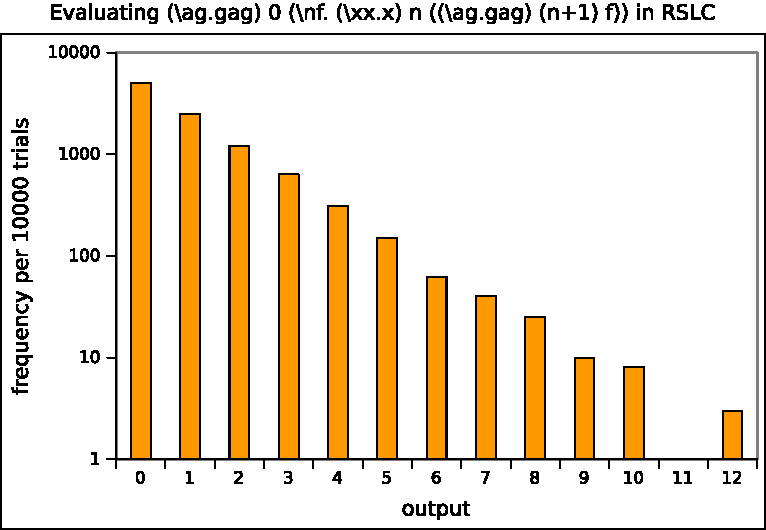
\includegraphics[width=0.48\textwidth]{rslc-naturals.pdf}
	\end{center}
	\caption{Computing random numbers with the term in Equation~\ref{eq:randomnat-fixed}. Log scale, lower is better. (I couldn't show $13$ because it showed up 0 times, and $\mathsf{log}~0 = -\infty$.)}
	\label{fig:nats}
\end{figure}

\subsection{Uniform random number generation}
\label{sec:uniform}

\newcommand{\thing}[1]{\textcolor{Fuchsia}{#1}}

The next thing I wanted to do was compute random numbers with a uniform distribution. Previously we were just selecting between two possible bindings for $x$, statically defined in the program text. I wondered, ``can I dynamically generate a term with $n$ shadow-bindings\footnote{Shadow binding: Sor/Wiz 3, Complete Arcane. Will save negates.} that causes a variable to have $n$ expressions in its $\rep{e}$ list?'' Something like:
\[
\thing{(\lambda x. (\lambda x. \dots (\lambda x.x)))}~0~1~2~\dots~n
\]
Of course this was where I had to iron out all the crazy parts in the previous sections, but since I already presented it in a manner consistent with it ain't being no thang, I'm going to make this part look easy:
% Y2 (\x.x) N (\tn. case n of 0 => (\f. t 0) | S(n2) => (\f. Y2 ((\x.t)n) n2 f))

\begin{center}
\begin{tabular}{rcl}
$\rho$ & = &
\hspace{-1em}\multirow{4}{*}{
\begin{tabular}{lllll}
\multicolumn{5}{l}{$\lambda \thing{\bf t}. \lambda n.$} \\
& \multicolumn{4}{l}{$\mathsf{case}~n~\mathsf{of}$} \\
&& $\Zero$ & $\Rightarrow$ & $\lambda f.~\thing{\bf t}~\Zero$ \\
&& $\Suc{n_2}$ &$\Rightarrow$& $\lambda f.~\Yab~\thing{((\lambda x.{\bf t})~n)}~n_2~f$
\end{tabular}
}
\\
&&\\
&&\\
&&\\
&&\\
$\mathsf{rand}[0,N]$ &=& $\Yab~\thing{(\lambda x.x)}~N~\rho$
\end{tabular}
\end{center}

The variable $\thing{\bf t}$ accumulates ``$\lambda x$''s as $\rho$ recurses (in the $\Suc{n_2}$ case). You might ask: why does the $\lambda f$ need to be inside the $\mathsf{case}$ statement?
Because otherwise in {\sc Eval-Case-2}$n_2$ would get captured in the thing substituted for $f$.

A brief, very condensed, evaluation run-through:

\begin{center}
\begin{tabular}{lll}
$\mathsf{rand}[0,2]$ &
= & $\Yab~\thing{(\lambda x.x)}~2~\rho$ \\
& $\mapsto^*$ & $\Yab~\thing{((\lambda x.(\lambda x.x))~2)}~1~\rho$ \\
& $\mapsto^*$ & $\Yab~\thing{((\lambda x.(\lambda x.(\lambda x.x))~2)~1)}~0~\rho$ \\
& $\mapsto^*$ & $((\lambda x.(\lambda x.(\lambda x.x))~2)~1)~0$ \\
& $\mapsto^*$ & $\subst{0}{x}x[1,2]$
\end{tabular}
\end{center}

\section{Deterministic Programming with RSLC}

Got here. Up until now I showed how random scope adds inherent nondeterminism that can be harnessed to simulate dice anda make silly graphs. The other thing Sully didn't believe would be possible was writing deterministic RSLC programs that {\em avoid} using ``the feature''.

In the last section I already introduced the capture-free Y combinator(s). Implementing addition using that is no trouble:

\newcommand{\addition}{\maltese}
\begin{center}
\begin{tabular}{rcl}
$\addition$ & = &
\hspace{-1em}\multirow{4}{*}{
\begin{tabular}{lllll}
\multicolumn{5}{l}{$\lambda m. \lambda n.$} \\
& \multicolumn{4}{l}{$\mathsf{case}~m~\mathsf{of}$} \\
&& $\Zero$ & $\Rightarrow$ & $\lambda f.~n$ \\
&& $\Suc{m'}$ &$\Rightarrow$& $\lambda f.~\Suc{\Yab~m'~n~f}$
\end{tabular}
}
\\
&&\\
&&\\
&&\\
&&\\
$\mathsf{add}~M~N$ &=& $\Yab~M~N~\addition$
\end{tabular}
\end{center}

But it turns out that multiplication, which uses addition, winds up needing the eager \textsf{let} construct. Among the several ways to implement it fully lazily, some introduce accidental randomness by letting some of \textsf{times}'s variables get captured, and others simply cause my implementation to run out of stack space or start swapping to disk when evaluating. Uh, anyway, here it is.

\newcommand{\multiplication}{\bigstar}
\newcommand{\multx}{\hat{x}}
\newcommand{\multm}{\hat{m}}
\newcommand{\multn}{\hat{n}}
\newcommand{\multf}{\hat{f}}
\newcommand{\multmm}{\hat{m}'}
\begin{center}
\begin{tabular}{rcl}
$\multiplication$ & = &
\hspace{-1em}\multirow{6}{*}{
\begin{tabular}{lllll}
\multicolumn{5}{l}{$\lambda \multm. \lambda \multn.$} \\
& \multicolumn{4}{l}{$\mathsf{case}~\multm~\mathsf{of}$} \\
&& $\Zero$ & $\Rightarrow$ & $\lambda \multf.~\Zero$ \\
&& $\Suc{\multmm}$ &$\Rightarrow$& $\lambda \multf.$ \\
&&
\multicolumn{3}{l}{
\begin{tabular}{lll}
& \textsf{let} & $\multx~=~\Yab~\multmm~\multn~\multf$ \\
& \textsf{in} & $\mathsf{add}~\multx~\multn$
\end{tabular}
}
\end{tabular}
}
\\
&&\\
&&\\
&&\\
&&\\
&&\\
&&\\
$\mathsf{times}~M~N$ &=& $\Yab~M~N~\multiplication$
\end{tabular}
\end{center}
Note that since $\mathsf{times}$ refers to $\mathsf{add}$, $\mathsf{times}$'s variable names must have different names. I put hats on them.

Here's the factorial function:
\newcommand{\factorial}{\textbf{!}}
\newcommand{\factx}{\mathring{x}}
\newcommand{\factn}{\mathring{n}}
\newcommand{\factf}{\mathring{f}}
\newcommand{\factnn}{\mathring{n}'}
\begin{center}
\begin{tabular}{rcl}
$\factorial$ & = &
\hspace{-1em}\multirow{6}{*}{
\begin{tabular}{lllll}
\multicolumn{5}{l}{$\lambda \factn.$} \\
& \multicolumn{4}{l}{$\mathsf{case}~\factn~\mathsf{of}$} \\
&& $\Zero$ & $\Rightarrow$ & $\lambda \factf.~\Suc{\Zero}$ \\
&& $\Suc{\factnn}$ &$\Rightarrow$& $\lambda \factf.$ \\
&&
\multicolumn{3}{l}{
\begin{tabular}{lll}
& \textsf{let} & $\factx~=~\Ya~\factnn~\factf$ \\
& \textsf{in} & $\mathsf{times}~\factn~\factx$
\end{tabular}
}
\end{tabular}
}
\\
&&\\
&&\\
&&\\
&&\\
&&\\
&&\\
$\mathsf{fact}~N$ &=& $\Ya~N~\factorial$
\end{tabular}
\end{center}

\newcommand{\fst}{\mathsf{fst}}
\newcommand{\snd}{\mathsf{snd}}
To compute fibonacci numbers, I used the standard Church encoding for pairs:
\begin{eqnarray*}
(e_1, e_2) &=& \lambda b.~b~e_1~e_2 \\
\fst~e &=& e (\lambda x.\lambda y. x) \\
\snd~e &=& e (\lambda x.\lambda y. y) \\
\end{eqnarray*}
Hence:
\newcommand{\fib}{\Phi}
\newcommand{\fibxa}{\tilde{x}_1}
\newcommand{\fibxb}{\tilde{x}_2}
\newcommand{\fibn}{\tilde{n}}
\newcommand{\fibf}{\tilde{f}}
\newcommand{\fibp}{\tilde{p}}
\newcommand{\fibnn}{\tilde{n}'}
\begin{center}
\begin{tabular}{rcl}
$\fib$ & = &
\hspace{-1em}\multirow{6}{*}{
\begin{tabular}{lllll}
\multicolumn{5}{l}{$\lambda \fibn.$} \\
& \multicolumn{4}{l}{$\mathsf{case}~\fibn~\mathsf{of}$} \\
&& $\Zero$ & $\Rightarrow$ & $\lambda \fibf.~(\Zero,~\Suc{\Zero})$ \\
&& $\Suc{\fibnn}$ &$\Rightarrow$& $\lambda \fibf.$ \\
&&
\multicolumn{3}{l}{
\begin{tabular}{lll}
& \textsf{let} & $\fibp~=~\Ya~\fibnn~\fibf$ \\
& & $\fibxa~=~\fst~\fibp$ \\
& & $\fibxb~=~\snd~\fibp$ \\
& \textsf{in} & $(\fibxb,~\mathsf{add}~\fibxa~\fibxb)$
\end{tabular}
}
\end{tabular}
}
\\
&&\\
&&\\
&&\\
&&\\
&&\\
&&\\
&&\\
&&\\
$\mathsf{fib}~N$ &=& $\Ya~N~\fib$
\end{tabular}
\end{center}

At this point I could include some addition and multiplication tables like the kind you saw in 3rd grade, but it would be no surprise.
Suffice to say that it works.

\section{Applications}

\begin{figure}[t]
	\begin{center}
	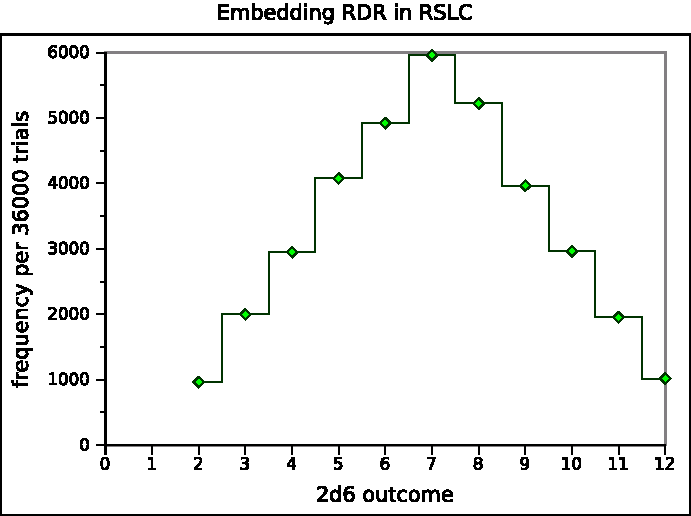
\includegraphics[width=0.48\textwidth]{rslc-rdr.pdf}
	\end{center}
	\caption{RSLC is a generalization of the Random Distance Run~\cite{rdr}.}
	\label{fig:rdr}
\end{figure}

\begin{figure}[t]
	\begin{center}
	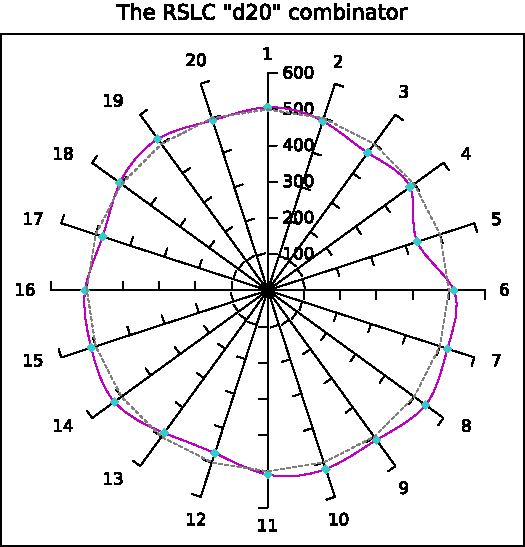
\includegraphics[width=0.40\textwidth]{rslc-d20.pdf}
	\end{center}
	\caption{RSLC can also be used to implement popular role-playing games.}
	\label{fig:d20}
\end{figure}

Now that I showed in an abstract sense how RSLC can be used to express popular computations from conventional lambda calculus as well as some novel random programming techniques, let's do a real-world application.
Using the uniform combinator from Section~\ref{sec:uniform}, we can make standard dice for any nonzero number of sides:

\begin{eqnarray*}
	\mathsf{d}(\Suc{N}) &=& \mathsf{add}~1~\mathsf{rand}[0,N] \\
       2\mathsf{d}(\Suc{N}) &=& \mathsf{let}~x=\mathsf{add}~\mathsf{rand}[0,N]~\mathsf{rand}[0,N] \\
	&& \mathsf{in}~\mathsf{add}~2~x \\
       3\mathsf{d}(\Suc{N}) &=& \mathsf{let}~x=\mathsf{add}~\mathsf{rand}[0,N]~\mathsf{rand}[0,N] \\
	&& \mathsf{in}~\mathsf{let}~y=\mathsf{add}~x~\mathsf{rand}[0,N] \\
	&& \mathsf{in}~\mathsf{add}~3~y
\end{eqnarray*}

For $N = 5$, using the $2\mathsf{d}(\Suc{N})$ combinator (more commonly known as $2\mathsf{d}6$), we obtain a random distribution equivalent to the one employed in the Random Distance Run~\cite{rdr}, as shown in Figure~\ref{fig:rdr}.

The value $N = 19$ yields the $\mathsf{d}20$ combinator, which generates the random distribution shown in Figure~\ref{fig:d20}. Prior work has shown this combinator to be quite useful in tabletop roleplaying games~\cite{dnd-mm,dnd-phb,dnd-dmg}.

\section{Theoretical Concerns}

Some programming language theoreticians will speak of the so-called ``Frame Rule'', which expresses abstraction: if a property $P$ holds for a certain function $f$, then in another function $g$ which invokes $x$, if $P(x)$ implies $P(g)$, then $P([f/x]g)$.

In the context of RSLC, we scoff at this rule.

\section{Concluding Remarks}

RSLC is an extension to standard un(i)typed lambda calculus in which substitution is essentially completely broken. However, since substitution is broken in a particularly careful way, it is possible to write interesting programs that make use of the language's built-in nondeterminism.
Furthermore, I showed that it is still possible to write a bunch of deterministic programs that are commonly used as examples/proofs-of-concept, as long as you put silly hats on some of your variables.

I believe you could extend RSLC's substitution schema to a typed lambda calculus, and furthermore if it only substitutes for variables of the same type, it would even be type-safe.

My implementation of RSLC in Haskell is available at \url{https://github.com/bblum/sigbovik/blob/master/RSLC/RSLC.hs}.

\bibliographystyle{alpha}
\bibliography{paper}

\newpage

\appendix

\section{Discussion of Substitution Rules}
\begin{figure*}[t]
	\fbox{$\subst{e_0}{x}{e}$}
	\TypeRules{
		\SubstLamCapture \qquad \SubstLam \qquad
		\SubstApp \\
		\SubstVarX \qquad \SubstVarY \\
		\SubstCaseCapture \\ \SubstCase \\
		\SubstZero \qquad \SubstSuc \\
		\SubstLetCapture \qquad \SubstLet
	}
	\fbox{$\capture{e_0}{x}{e}$}
	\TypeRules{
		\CaptureLam \qquad \CaptureApp \qquad
		\CaptureVarX \qquad \CaptureVarY \\
		\CaptureCase \\
		\CaptureZero \qquad \CaptureSuc \qquad \CaptureLet
	}
	\caption{Complete RSLC substitution and capture rules.}
	\label{fig:subst-complete}
\end{figure*}

\end{document}
